\documentclass[a4paper, 11pt, table]{article}

\usepackage[utf8]{inputenc}
\usepackage[english]{babel}
\usepackage[table]{xcolor}
\usepackage{graphicx}
\usepackage{tikz}
\usetikzlibrary{calc}
\usepackage{float}
\usepackage{pifont,mdframed}
\usepackage{subfig}
\usepackage{amsmath}
\usepackage{siunitx}
\usepackage{caption}
\usepackage{lscape}
\usepackage{pifont}
\usepackage{footnote}
\makesavenoteenv{tabular}

\usepackage[
backend=biber
]{biblatex}
\addbibresource{references.bib}

\definecolor{Gray}{gray}{0.9}
\definecolor{LabelColor}{gray}{0.0}
\definecolor{clno}{RGB}{212, 59, 59}
\definecolor{clyes}{RGB}{12, 150, 12}
\definecolor{linux}{RGB}{255, 186, 249}
\definecolor{windows}{RGB}{186,215, 255}
\definecolor{macos}{gray}{0.9}  
\newcommand{\cmark}{\ding{51}}%
\newcommand{\xmark}{\ding{55}}%
\newcommand{\ymark}{\textcolor{clyes}{\cmark}}%
\newcommand{\nmark}{\textcolor{clno}{\xmark}}%

\graphicspath{ {img/} }

% warning environment
% It should not be included in final report
% http://tex.stackexchange.com/questions/8689/how-to-create-a-warning-box-like-this-see-the-figure-to-get-the-idea
\newenvironment{warning}
  {\par\begin{mdframed}[linewidth=2pt,linecolor=red]%
    \begin{list}{}{\leftmargin=1cm
                   \labelwidth=\leftmargin}\item[\Large\ding{43}]}
  {\end{list}\end{mdframed}\par}

\title{Convolutional neural networks for classification of transmission electron microscopy imagery}

\author{Sergii Gryshkevych}
\date{\today}

\begin{document}

\maketitle

\tableofcontents

\begin{abstract}
An abstract.
\end{abstract}

\section{Introduction}
This is my thesis job report. 

\section{Background}

\subsection{Problem description}

\subsubsection{Lamellarity}
Describe what is lamellarity and give references.
\begin{figure}[H]
\centering
\begin{tabular}{ccc}
	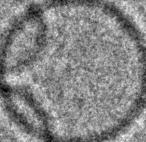
\includegraphics[height=2cm, keepaspectratio]{problem_description/lamellarity/uni} & 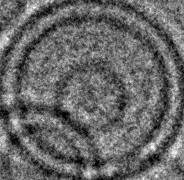
\includegraphics[height=2cm, keepaspectratio]{problem_description/lamellarity/multi} & 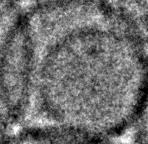
\includegraphics[height=2cm, keepaspectratio]{problem_description/lamellarity/uncertain} \\
	Unilamellar & Multiilamellar & Uncertain \\[6pt]
\end{tabular}
\caption{Lamellarity problem, 3 classes}
\end{figure}

\subsubsection{Encapsulation}
Describe drug delivery problem and give references.
\begin{figure}[H]
\centering
\begin{tabular}{ccc}
	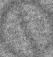
\includegraphics[height=2cm, keepaspectratio]{problem_description/packiging/full} & 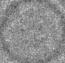
\includegraphics[height=2cm, keepaspectratio]{problem_description/packiging/empty} & 
\includegraphics[height=2cm, keepaspectratio]{problem_description/packiging/uncertain} \\
	Full & Empty & Uncertain \\[6pt]
\end{tabular}
\caption{Encapsulation problem, 3 classes}
\end{figure}

\subsection{The data set}

\begin{center}
\captionof{table}{Lamellarity problem}
\begin{tabular}{lrr}
\hline 
Unilamellar & 12368 & 87.29\% \\ 
Multilamellar & 1717 & 12,12\% \\ 
Uncertain & 84 & 0,59\% \\ 
\end{tabular} 
\end{center}

\begin{center}
\captionof{table}{Encapsulation problem}
\begin{tabular}{lrr}
\hline 
Full & 24255 & 97.34\% \\ 
Uncertain & 502 & 2.01\% \\ 
Empty & 161 & 0.65\% \\ 
\end{tabular} 
\end{center}


Here comes description of the data set. Describe images and features.

\subsubsection{Principal component analysis}

Features included in principal component analysis (PCA):
\begin{itemize}
\item Area
\item Circularity
\item Perimeter
\item Length
\item Maximum width
\item Signal to noise
\item M20
\item M02
\item M30
\item M03
\end{itemize}

\begin{figure}[H]
\centering
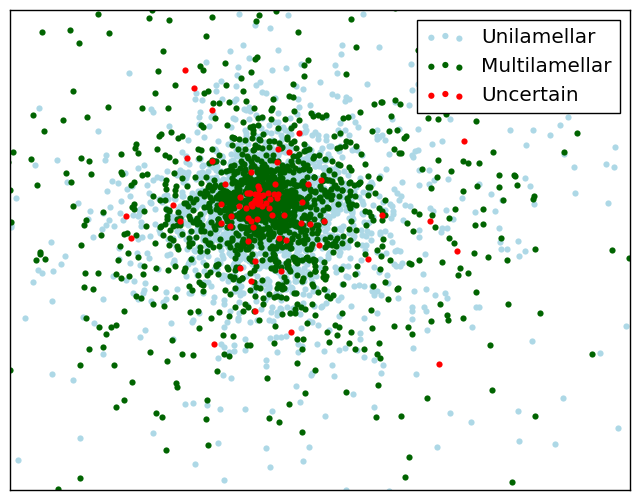
\includegraphics[scale=0.7]{pca/lamellarity.png}
\caption{PCA lamellarity problem. \\ Explained variance ration by first two components: 94.78\%, 3.39\%}
\end{figure}

\begin{figure}[H]
\centering
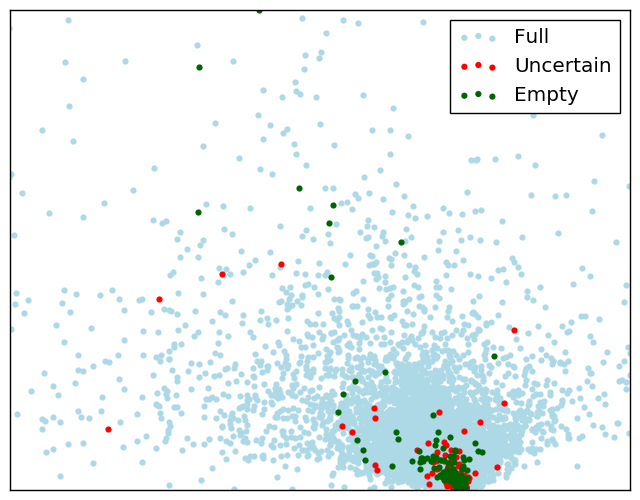
\includegraphics[scale=0.7]{pca/encapsulation.png}
\caption{PCA encapsulation problem. \\ Explained variance ration by first two components: 66.20\%, 19.96\%}
\end{figure}

\subsection{Imbalance problem}

Describe imbalance problem. Imbalance problem has been studied in~\cite{imbalanced-data}, ...
Give examples of domains where data is usually imbalanced. 

\section{Methodology}

\subsection{Convolutional Neural Networks}
Motivate use of convolutional neural networks, add a lot of references to~\cite{dl_book}
\subsection{Regularization}

Motivate need of regularization and describe problems that is solves. 
Reularization techniques that I have tried.

\subsubsection{Weight decay}

\begin{warning}
With weight decay many convolution kernels are equal to zero. 
\end{warning}

\begin{figure}[H]
\centering
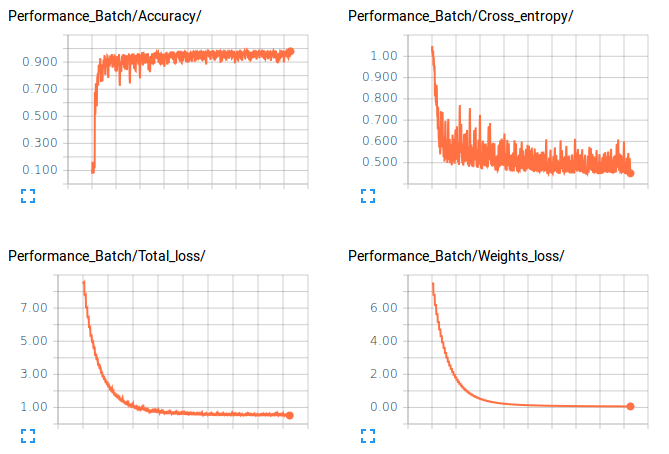
\includegraphics[scale=0.5]{weight_decay/performance.png}
\caption{Batch performance metrics}
\end{figure}

\begin{figure}[H]
\begin{tabular}{cc}
	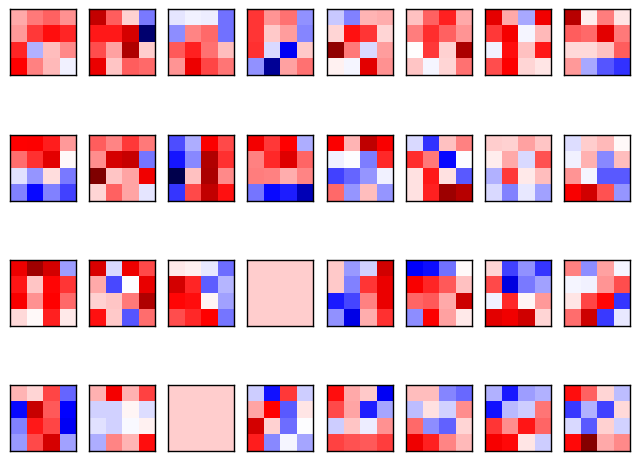
\includegraphics[scale=0.4]{weight_decay/filters1.png} & 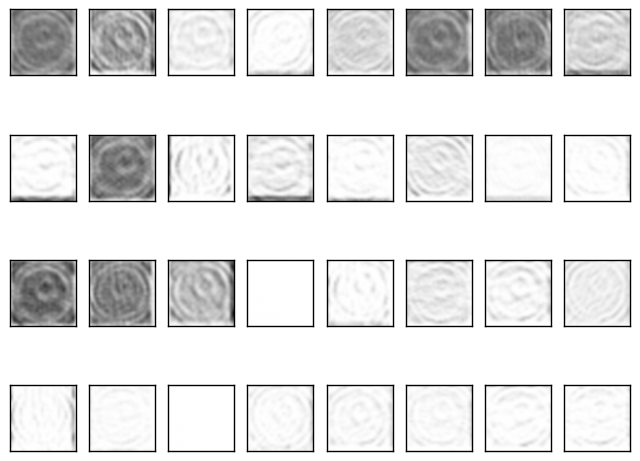
\includegraphics[scale=0.4]{weight_decay/conv1.png} \\
	Convolution kernels & Output \\[6pt]
\end{tabular}
\caption{First convolutional layer}
\end{figure}

\begin{figure}[H]
\begin{tabular}{cc}
	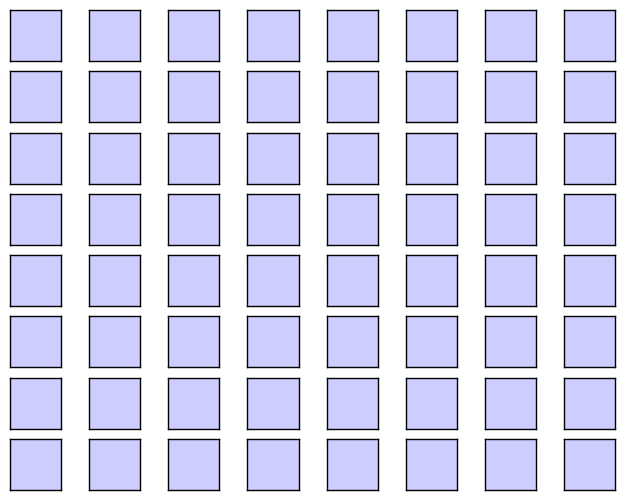
\includegraphics[scale=0.4]{weight_decay/filters2.png} & 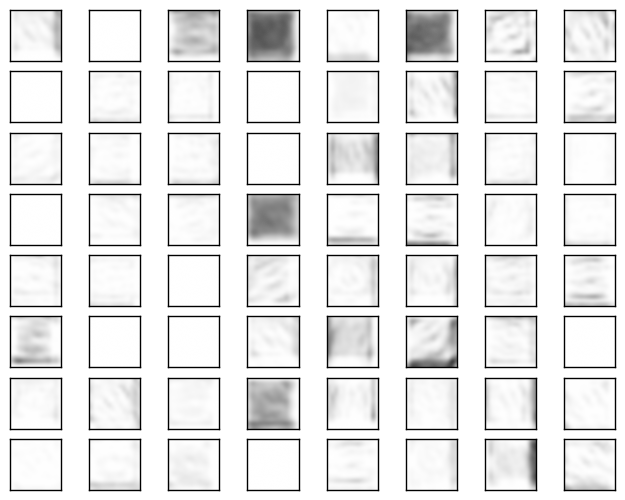
\includegraphics[scale=0.4]{weight_decay/conv2.png} \\
	Convolution kernels, channel 27 & Output (all 32 channels applied) \\[6pt]

\end{tabular}
\caption{Second convolutional layer}
\end{figure}

\subsubsection{Noise injection}
\begin{equation}
\label{eq:soft_targets}
x \leftarrow x \left( 1 - \epsilon \right) + \left(1 - x\right) \frac{\epsilon}{k - 1}
\end{equation}

\subsection{Data augmentation}
Motivate data augmentation and give references.

\subsubsection{Oversampling}
Minority classes have been oversampled in the following way:

\begin{itemize}
\item Rotation by 90, 180 and 270 degrees
\item Flipping
\item Rotation of flipped image by 90, 180 and 270 degrees
\end{itemize}

One flipping and six rotations increase number of samples by factor 7. Rotation values have been selected as multiples of \SI{90}{\degree} for performance reasons. Rotation by multiples of \SI{90}{\degree} does not require any interpolation and can be performed efficiently.

\subsubsection{Undersampling}
Majority class has been undersampled by 20\%. This means that during each epoch 20\% of randomly selected examples of majority class are ignored during training.

\subsubsection{SMOTE}
Synthetic Minority Over-sampling Technique (SMOTE) is an over-sampling approach in which the minority class is over-sampled by creating “synthetic” examples rather than by over-sampling with replacement~\cite{smote_chawla}. 
Synthetic examples are generated by combining each minority class example with its randomly selected $k$ nearest neighbors, where $k$ is a parameter that depends on amount of required over-sampling.

\begin{warning}
Add figure of some liposome, its nearest neighbors and generated synthetic examples.
\end{warning}

\subsubsection{Synthetic data}
Synthetic and semi-synthetic alternative to real data have been discussed and evaluated in~\cite{ishaq_synthetic}. I also tried to generate synthetic data, train network on it and evaluate on real data. Performance was poor, much worse than training on over-sampled and semi-synthetic data produced by SMOTE. 

\begin{figure}[H]
\centering
\begin{tabular}{ccc}
	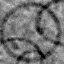
\includegraphics[scale=1.5]{synthetic/uni.png} & 
\includegraphics[scale=1.5]{synthetic/multi.png} & 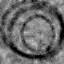
\includegraphics[scale=1.5]{synthetic/uncertain.png} \\
	Unilamellar & Multiilamellar & Uncertain \\[6pt]
\end{tabular}
\caption{Synthetic examples, lamellarity problem}
\end{figure}

\begin{warning}
Kommentar från Max: Det kan vara svårt att motivera en syntetiseringsmetod som inte grundar sig på statistiska mått på huvuddatan. Prova gärna att göra mindre rotationer, 10 grader eller så, använd gärna Lanczos-interpolering, du kan fråga Ida-Maria om referens för det (poängen är att Lanczos bibehåller textur-statistik mycket bättre än t ex linjärinterpolering).
\end{warning} 

\subsection{Loss function}

\begin{warning}
This section is taken from project report for Machine Learning course. How to cite it?
\end{warning}

The multi-class logarithmic loss function is a loss function that represents the price paid for inaccuracy of predictions in classification problems~\cite{rosasco}. The formula is:
\begin{equation}
loss = -\frac{1}{N} \sum_{i=1}^{N} \sum_{j=1}^{M} y_{i,j} log(p_{i,j})
\end{equation}

Where 
\begin{itemize}
\item N -- number of observations
\item M -- number of classes, it is five in our case
\item \textit{log} -- natural logarithm
\item $y_{i,j}$ -- is 1 if observation $i$ is in class $j$ and 0 otherwise
\item $p_{i,j}$ --  is the predicted probability that observation $i$ is in class $j$
\end{itemize}

In order to calculate multi-class logarithmic loss the classifier must assign a probability to each class rather than simply yielding the most likely class. This fact constitutes the main difference between accuracy and logarithmic loss. In order to consider a prediction as accurate, it is sufficient that classifier marks the correct class as the most likely one, no matter how confident the prediction is.

Figure~\ref{fig:logloss} shows log loss from a single class where predicted probability ranges from 0 (the completely wrong prediction) to 1 (the correct prediction). As predicted probability moves closer to 1, log loss decreases gently to 0. On the contrary, log loss increases rapidly as predicted probability moves towards zero. It is clear from Figure~\ref{fig:logloss} that the multi-class logarithmic loss heavily penalizes classifiers that are confident about an incorrect classification.

\begin{figure}[H]
\centering
\begin{tikzpicture}
  \node[inner sep=0pt] (A) {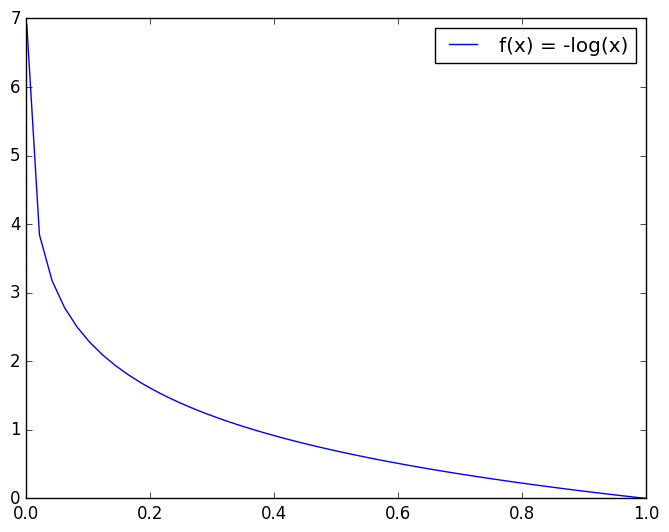
\includegraphics[width=0.8\textwidth]{log_loss}};
  \node[LabelColor] (B) at ($(A.south)!-.05!(A.north)$) {Predicted probability};
  \node[LabelColor,rotate=90] (C) at ($(A.west)!-.05!(A.east)$) {Log Loss};
\end{tikzpicture}
\caption{\label{fig:logloss} Log loss of a single class where predicted probability ranges from 0 to 1. }
\end{figure}

Consider an example of a binary classifier and let us take a look at the effect of various predictions for class membership probability. 
\begin{itemize}
\item Classification that assigns equal probabilities to both classes results in loss $-log(0.5)=0.6932$.  

\item Classification confident in the correct class results in loss $-log(0.9)=0.1054$.

\item Classification confident in the wrong class results in loss $-log(0.1)=2.3026$. 
\end{itemize}

In other words, the log loss function encourages moderate predictions. It is better to make all classifications neutral rather than make 50\% correct classifications and 50\% completely wrong predictions.


\subsubsection{Dropout}

\subsubsection{Early stopping}


\section{Implementation of CNN}

\subsection{Network visualization}

\begin{figure}[H]
\begin{tabular}{cc}
	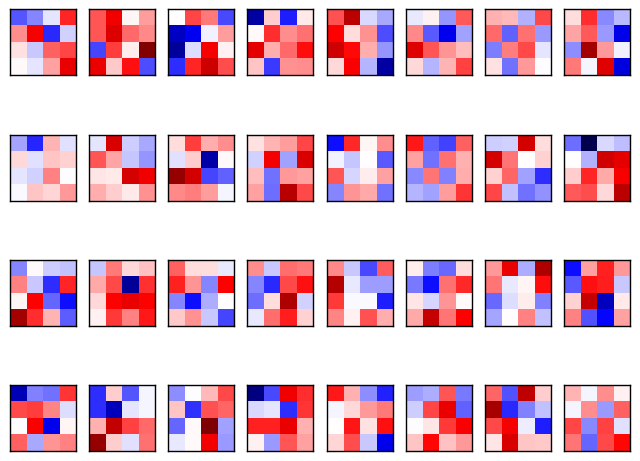
\includegraphics[scale=0.4]{conv_layers/filters1.png} & 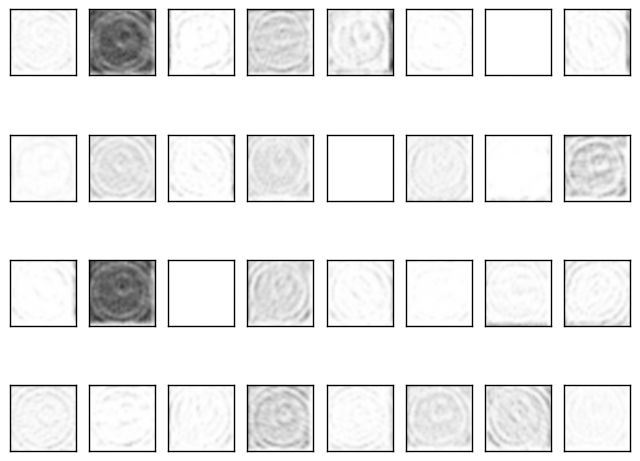
\includegraphics[scale=0.4]{conv_layers/conv1.png} \\
	Convolution kernels & Output \\[6pt]

\end{tabular}
\caption{First convolutional layer}
\end{figure}

\begin{figure}[H]
\begin{tabular}{cc}
	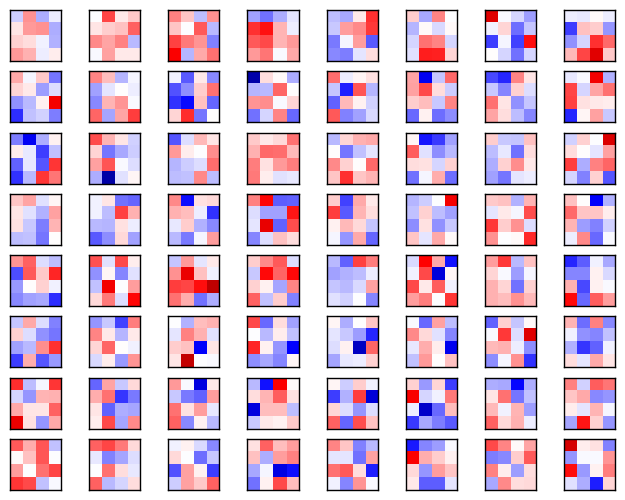
\includegraphics[scale=0.4]{conv_layers/filters2.png} & 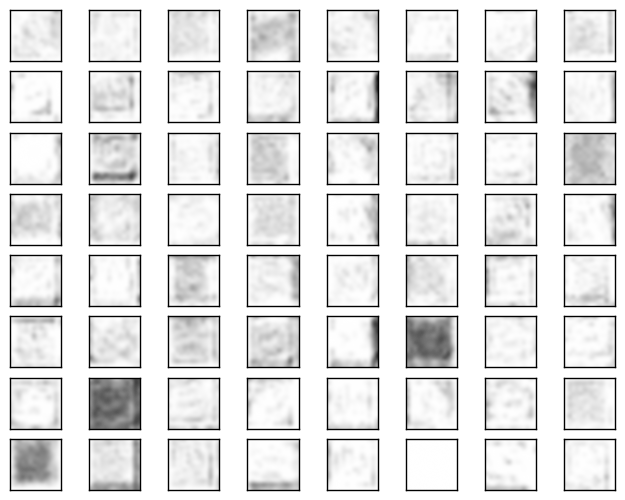
\includegraphics[scale=0.4]{conv_layers/conv2.png} \\
	Convolution kernels, first channel & Output \\[6pt]

\end{tabular}
\caption{Second convolutional layer}
\end{figure}

\subsection{Review of deep learning software libraries}

Deep learning software tool have been benchmarked in~\cite{benchmarking_dl_tools}

\begin{landscape}
\begin{center}
\captionof{table}{Comparison of characteristics of deep learning frameworks}
\begin{tabular}{lccccccccl}
\hline 
 & \multicolumn{2}{c}{\cellcolor{linux}Linux} & \multicolumn{2}{c}{\cellcolor{windows}Windows} & \multicolumn{2}{c}{\cellcolor{macos}Mac OS} & \multicolumn{2}{c}{Language bindings} &  \\ 
 & \cellcolor{linux}CPU & \cellcolor{linux}GPU & \cellcolor{windows}CPU & \cellcolor{windows}GPU & \cellcolor{macos}CPU & \cellcolor{macos}GPU & Python & C++ & License\\ 
\hline 
Caffe & \ymark & \ymark & \ymark & \ymark & \ymark & \ymark & \ymark & \nmark & BSD 2\\ 
cntk & \ymark & \ymark & \ymark & \ymark & \nmark & \nmark & \ymark & \ymark & Custom\footnote{Allows commercial use \textcolor{red}{reference}} \\ 
Keras & \ymark & \ymark & \nmark & \nmark & \ymark & \nmark & \ymark & \nmark & MIT \\ 
Lasagne & \ymark & \ymark & \ymark & \ymark & \ymark & \ymark & \ymark & \nmark & MIT \\ 
mxnet & \ymark & \ymark & \ymark & \ymark & \ymark & \ymark & \ymark & \ymark & Apache 2.0 \\ 
nolearn & \ymark & \ymark & \ymark & \ymark & \ymark & \ymark & \ymark & \nmark & MIT \\ 
Tensorflow & \ymark & \ymark & \nmark & \nmark & \ymark & \nmark & \ymark & \ymark & Apache 2.0 \\ 
Theano & \ymark & \ymark & \ymark & \ymark & \ymark & \ymark & \ymark & \nmark & BSD 3\\ 
\end{tabular} 
\end{center}

\begin{center}
\captionof{table}{Comparison of popularity of deep learning frameworks}
\begin{tabular}{lrrrrr}
\hline 
 & \multicolumn{4}{c}{Github} & Stackoverflow \\ 
 & Contributors & Stars & Forks & Subscribers & Questions \\ 
\hline 
Caffe & 208 & 12349 & 7513 & 1559 & 1038 \\ 
cntk & 77 & 6181 & 1343 & 688 & 12 \\ 
Keras & 257 & 8044 & 2470 & 639 & 444 \\ 
Lasagne & 51 & 2452 & 673 & 202 & 153 \\ 
mxnet & 174 & 4969 & 1887 & 559 & 22 \\ 
nolearn & 9 & 718 & 203 & 52 & 44 \\ 
Tensorflow & 380 & 31445 & 13414 & 2983 & 3275 \\ 
Theano & 251 & 4475 & 1609 & 424 & 1436 \\ 
\end{tabular} 
\end{center}



\end{landscape}

\section{Evaluation}

\subsection{ROC}

\subsection{Confusion matrix}

\begin{warning}
Problem with \textbf{Uncertain} class.
\end{warning}

\begin{center}
\captionof{table}{Lamellarity problem}
\begin{tabular}{lrrr}
\hline
 & Unilamellar & Uncertain & Multilamellar \\ 
\hline 
Unilamellar & 0.97 & 0.00 & 0.03 \\ 
Uncertain & 0.29 & 0.00 & 0.71 \\ 
Multilamellar & 0.04 & 0.00 & 0.96 \\ 
\end{tabular} 
\end{center}

\begin{center}
\captionof{table}{Packiging problem}
\begin{tabular}{lrrr}
\hline
 & Empty & Full & Uncertain \\ 
\hline 
Empty & 0.41 & 0.41 & 0.18 \\ 
Packed & 0.00 & 0.95 & 0.05 \\ 
Uncertain & 0.20 & 0.11 & 0.69 \\ 
\end{tabular} 
\end{center}

\subsection{K-fold cross validation}

\section{Results}

\section{Conclusion}

\section{Discussion}

\printbibliography

\end{document}
